%\documentclass[handout,aspectratio =169]{beamer}
\documentclass[presentation,aspectratio =169]{beamer}
\mode<presentation>
{
%  \usetheme{default}
   \usetheme[left]{Marburg}
  \usecolortheme{beaver}
  \usefonttheme{professionalfonts}  
  \setbeamertemplate{navigation symbols}{
  \insertframenumber/\inserttotalframenumber
  }
  \setbeamertemplate{caption}[numbered]
 } 

\setbeamertemplate{section in toc}[sections numbered]
\setbeamertemplate{subsection in toc}[subsections numbered]

  
\AtBeginSection[]
{
 \begin{frame}<beamer>
 \frametitle{Outline}
 \tableofcontents[currentsection]
 \end{frame}
}

%\addtobeamertemplate{navigation symbols}{}{%
%    \usebeamerfont{footline}%
%    \usebeamercolor[fg]{footline}%
%    \hspace{1em}%
%    \insertframenumber/\inserttotalframenumber
%}

\usepackage[english]{babel}
\usepackage[utf8x]{inputenc}
% \usepackage{graphicx}
\usepackage{array}
\usepackage{subfig}
\usepackage{tikz}
\usepackage{appendixnumberbeamer}
\usepackage{amssymb}
\usepackage{amsmath}
\usepackage{hyperref}
\usepackage{mathtools}
% \usepackage{lipsum}
\usepackage[makeroom]{cancel}
%\usepackage{minted}
\usepackage{bm}  
% \usepackage{xmpmulti}
\usepackage{algorithm}
\usepackage{algorithmic}
\usepackage{color}
\usepackage{multicol}
\usepackage{comment}
\usepackage{calc}  
%\usepackage[dvipsnames]{xcolor}


\definecolor{CMaroon}{RGB}{139,31,65}
\definecolor{VSunset}{RGB}{247,144,30} %This is really "Virginia Sunset" %\definecolor{VSunset}{RGB}{255,102,0} 
\definecolor{HStone}{RGB}{109,106,117} 
 \makeatletter
\setbeamertemplate{sidebar canvas \beamer@sidebarside}[vertical shading][top=VSunset!60,bottom=VSunset!90]
\makeatother
\setbeamercolor{palette sidebar secondary}{fg=CMaroon}
\setbeamercolor{section in sidebar shaded}{fg=black}
\setbeamercolor{subsection in sidebar shaded}{fg=black}
\setbeamercolor{subsection in sidebar}{fg=CMaroon}
\setbeamerfont{section in sidebar}{series=\bfseries}
\setbeamerfont{subsection in sidebar shaded}{series=\bfseries}
\makeatletter


\AtBeginLecture{
\frame{
\begin{center}
	\Large Today's Lecture: \\  
	\vspace{1cm}
	\insertlecture
\end{center}
}
}

% set sidebar with ToC


\graphicspath{{./logos/}{./figs/}}

%\subsection{} % A subsection can be created just before a set of slides with a common theme to further break down your presentation into chunks
\makeatletter
\newcommand{\setnextsection}[1]{%
  \setcounter{section}{\numexpr#1-1\relax}%
  \beamer@tocsectionnumber=\numexpr#1-1\relax\space}
\makeatother

\newcommand{\mb}[1]{\mathbf{#1}}
\newcommand{\bs}[1]{\boldsymbol{#1}}
\newcommand{\var}{\mathbb{V}\textrm{ar}}
\newcommand{\cov}{\mathbb{C}\textrm{ov}}
\newcommand{\ex}{\mathbb{E}}
\newcommand{\wex}{\widehat{\mathbb{E}}}
\newcommand{\readingslide}[1]{\textcolor{blue}{[#1]}}
\newcommand{\reviewslide}[1]{\colorbox{green!60}{#1}}
\newcommand{\defterm}[1]{\textcolor{red}{#1}}
\newcommand{\credit}[2]{\begin{flushright}
 \tiny (#1 Courtesy of #2)
\end{flushright}}
%\tikz\draw (0,0) rectangle (0.99\textwidth,0.42\textheight);
\newcounter{enumiCont}


\newcommand\blfootnote[1]{%
  \begingroup
  \renewcommand\thefootnote{}\footnote{#1}%
  \addtocounter{footnote}{-1}%
  \endgroup
}

\newcommand{\outlinechapter}[1]{
  \frame{\frametitle{#1}\tableofcontents[currentsection,currentsubsection]}
}

\newlength{\fullcolwidth}
\setlength{\fullcolwidth}{0.95\textwidth}

\newcommand{\figfactor}{0.85}
\newcommand{\heightfigfactor}{1.15}


\newcommand{\topicpage}[1]{
\begin{frame}{}
\begin{center}
{\LARGE \color{blue}#1}
\end{center}
\end{frame}
}

%\tikz\draw (0,0) rectangle (0.99\textwidth,0.42\textheight);
%\newcounter{enumiCont}

\title[AOE 5984: UQML]{AOE5984: \\Machine Learning and Uncertainty Quantification \\
for Scientists and Engineers\\
Independence Study}
\author[Hongsheng Wang]{Hongsheng Wang
   \\ Ph.D Student
}
\institute{Department of Mining and Minerals Engineering \\ Virginia Tech \\
  \medskip
  \bigskip
  
\includegraphics[height=20mm,keepaspectratio]{logo} \vspace{5mm}
  
\includegraphics[height=20mm,keepaspectratio]{text}
}
\date{~}


\begin{document}



\begin{frame}[noframenumbering]
  \titlepage
\end{frame}

%%% Local Variables:
%%% mode: latex
%%% TeX-master: "UQML-main-handout"
%%% End:



\part{Advanced Intro to Probability}
\setnextsection{1}


\section{Introduction to Importance Sampling}
\outlinechapter{Independence Study: Importance Sampling}

% !TEX root = ../UQML-main-handout.tex
% !TEX root = ../UQML-main-beamer.tex

\subsection{Theory of Importance Sampling}

% \begin{frame}[noframenumbering]
  \titlepage
\end{frame}

%%% Local Variables:
%%% mode: latex
%%% TeX-master: "UQML-main-handout"
%%% End:

\lecture{Introduction to Importance Sampling}{Intro-Importance-Sampling}

\begin{frame}{Monte Carlo Methods Review}

\begin{quote}
Monte Carlo Method is the art of approximating an expectation by the sample mean of a function of simulated random variables.\\
If $X$ is discrete:\\
\[\mathbb{E}(f(X))=\sum_{x \in \mathcal{X}} f(x) p_{X}(x)\]

If $X$ is continuous:\\
\[\mathbb{E}(f(X))=\int_{x \in \mathcal{X}} f(x) p_{X}(x) d x\]
\begin{flushright}
\textbf{}\\

\end{flushright}
\end{quote}
\end{frame}

\begin{frame}{Monte Carlo Methods}
Take the samples $X\sim p$ and we could have the Monte Carlo estimate:\\
\[\widetilde{f_{n}}(x)=\frac{1}{n} \sum_{i=1}^{n} f\left(x_{i}\right)\]
Notice that, $\widetilde{f_{n}}(x)$ is unbiased for $\mathrm{E}(f(X))$:\\
\[\mathbb{E}\left(\widetilde{f_{n}}(X)\right)=\mathbb{E}\left(\frac{1}{n} \sum_{i=1}^{n} f\left(X_{i}\right)\right)=\frac{1}{n} \sum_{i=1}^{n} \mathbb{E}\left(f\left(X_{i}\right)\right)=\mathbb{E}(f(X))\]
\end{frame}

\begin{frame}{Monte Carlo Method}

Monte Carlo Methods are widely used:

\begin{itemize}
\item Probability Approximation;\\
\item Simulate Distribution;\\ 
\item A Discrete Sum over Latent Variables.
\item $...$
\end{itemize}
Though Monte Carlo Methods are easy to formulate a quantity as an expectation, it is quite another thing to actually have the Monte Carlo estimator provide you with good estimates in a reasonable amount of computing time.\\
Typically, a \textcolor{red}{better} Monte Carlo estimator has smaller variance with the same computational effort than others.

\end{frame}

\begin{frame}{Pilot Example -- Probability of Cauchy Density}

\begin{quote}
Suppose that we are interested in the quantity of the probability $p$, which is a Cauchy $C(0,1)$ variable is larger than 2, described as the equation below:\\
\[
p(X>2) = \int_{2}^{+\infty }\frac{1}{\pi (1+x^{2})}dx
\]
Assume we can't integrate directly (of course we can use $arctan$ function) and we have to obtain $p$ by sampling the density.\\
What is the estimate and variance of estimator?
\begin{flushright}
\textbf{}\\

\end{flushright}
\end{quote}
\end{frame}

\begin{frame}{Different Estimators -- I and II}

\[
\boxed{
p(X>2) = \int_{2}^{+\infty }\frac{1}{\pi (1+x^{2})}dx}
\]

\begin{itemize}
\item I: The simplest model (naive sampling):\\ \[
\hat{p}_{1}=\frac{1}{m}\sum_{j=1}^{m}\mathbb{I}_{X_{j}>2}
\]
where, $X_{1}$ ,$...$ , $X_{n}$ $\sim$ $C(0,1)$ and i.i.d., and $\mathbb{I}$ is an indicator function. 
\item II: Taking into account the symmetric nature of $C(0,1)$:\\ \[\hat{p}_{2} = \frac{1}{2m}\sum_{j=1}^{m}\mathbb{I}_{\left | X_{j} \right |>2}\]

\end{itemize}
\end{frame}

\begin{frame}{Pilot Example -- Probability of Cauchy Density [1]}

\begin{figure}[ht]
		  \centering
          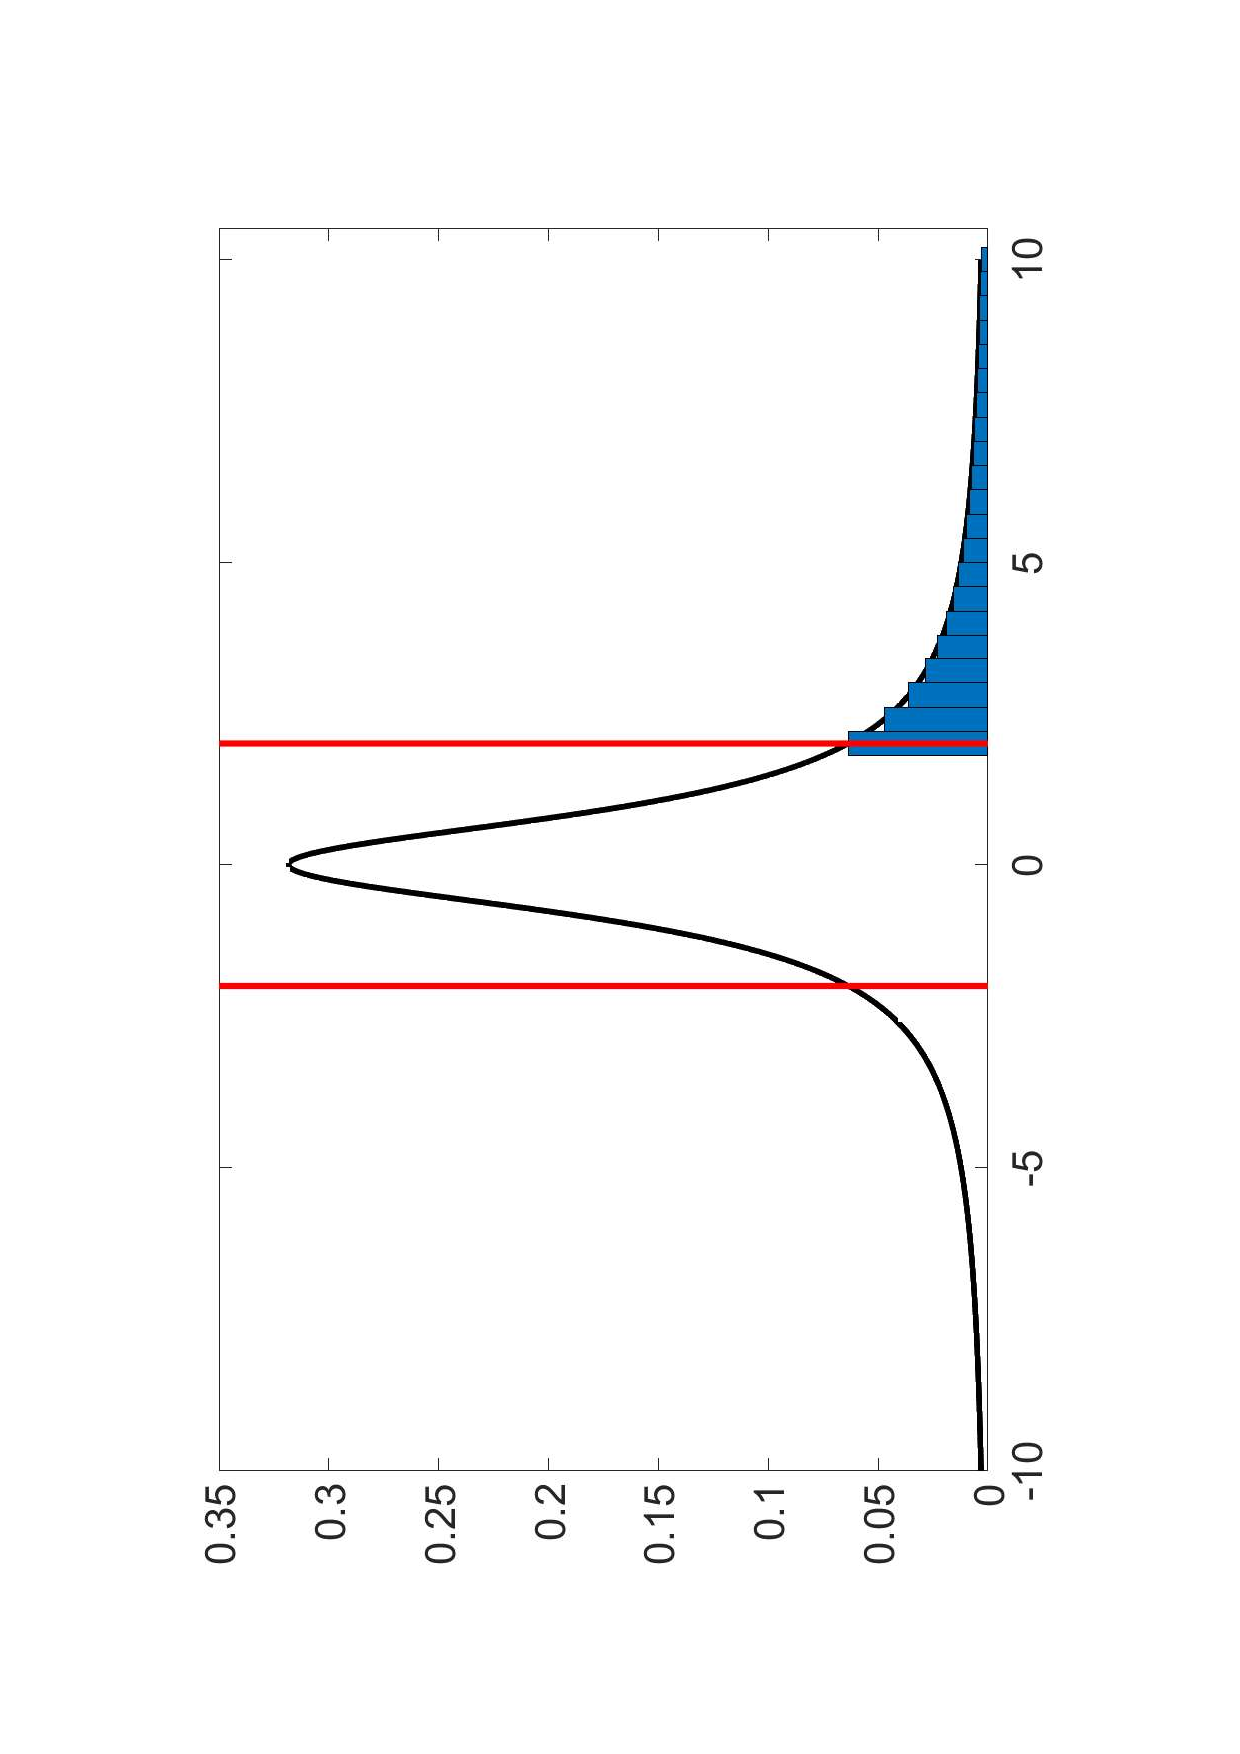
\includegraphics[scale = 0.3, angle = 270]{CauchyPDF12.pdf}
           \caption{Cauchy Distribution Estimator 1 and 2}
\end{figure}

\end{frame}

\begin{frame}{Different Estimators -- III}

\[
\boxed{
p(X>2) = \int_{2}^{+\infty }\frac{1}{\pi (1+x^{2})}dx}
\]

\begin{itemize}
\item The integral can be considered to be the expectation of :\\ \[h(X) = \frac{2}{\pi(1+X^{2})}\] \[\hat{p}_{3}=\frac{1}{2}-\frac{1}{m}\sum_{j=1}^{m}h(U_{j})\] \\ Where,  $U_{j}\sim \mathcal{U} {\left[ 0, 2  \right]}$ is a uniform distribution. 

\end{itemize}

\begin{alertblock}{Change of Measure}
The change of measure lead to a change of support from $[2, \infty]$ to $[0, 2]$. \alert{Why}?
\end{alertblock}

\end{frame}

\begin{figure}[ht]
		  \centering
          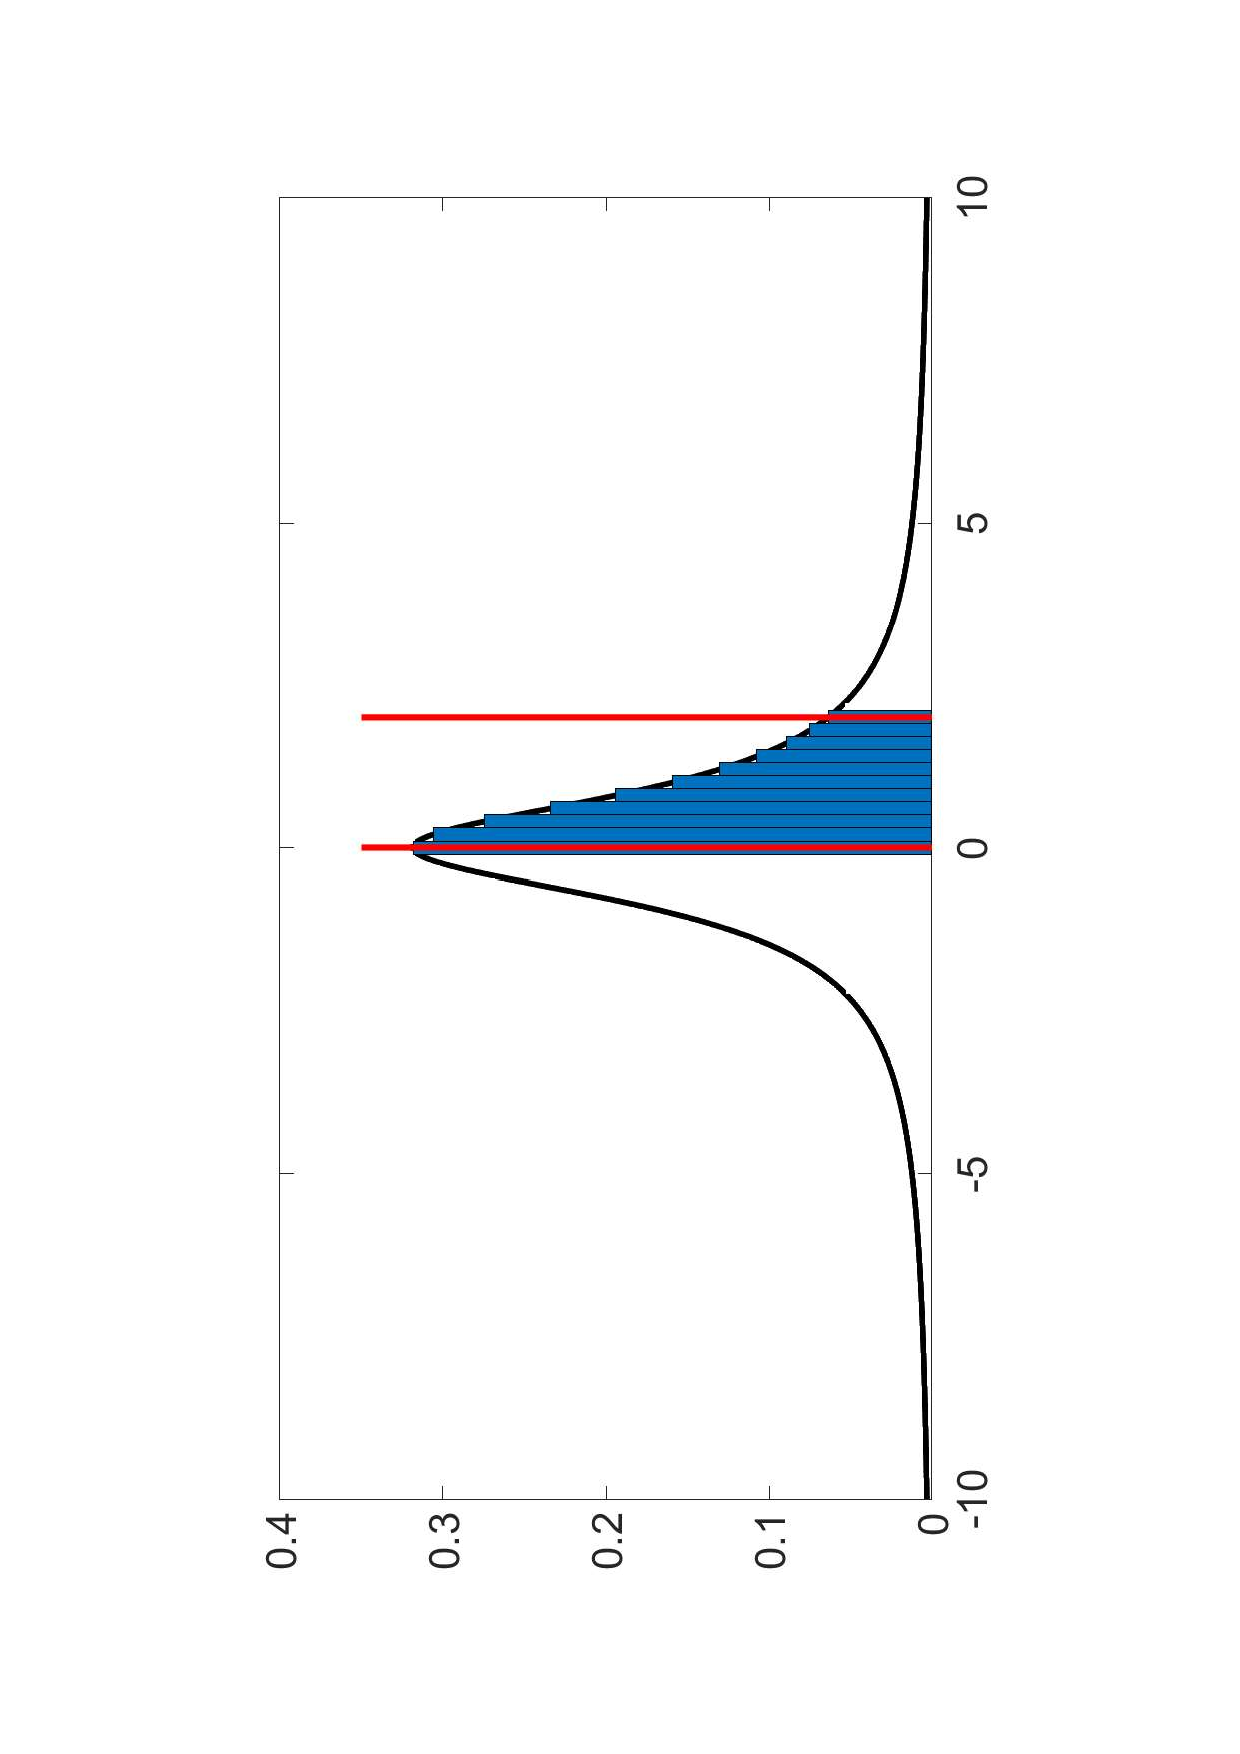
\includegraphics[scale = 0.3, angle = 270]{CauchyPDF3.pdf}
           \caption{Cauchy Distribution Estimator 3}
\end{figure}

\begin{frame}{Different Estimator -- IV}

\[
\boxed{
p(X>2) = \int_{2}^{+\infty }\frac{1}{\pi (1+x^{2})}dx}
\]

\alert{Change of measure from $p(x)$ to $p(y)$. Show!}

\begin{itemize}
\item Assume $y = x^{-1} $, the integral can be considered to be the expectation of:\\ \[h(Y) = \frac{2}{\pi (1+Y^{2})}\] \[\hat{p}_{4}=\frac{1}{4m}\sum_{j=1}^{m}h(Y_{j})\] \\ Where,  $Y_{j}\sim \mathcal{U} {\left [ 0, \right \frac {1}{2}]}$. 

\end{itemize}
\end{frame}

\begin{frame}{Pilot Example -- Probability of Cauchy Density}

\begin{figure}[ht]
		  \centering
          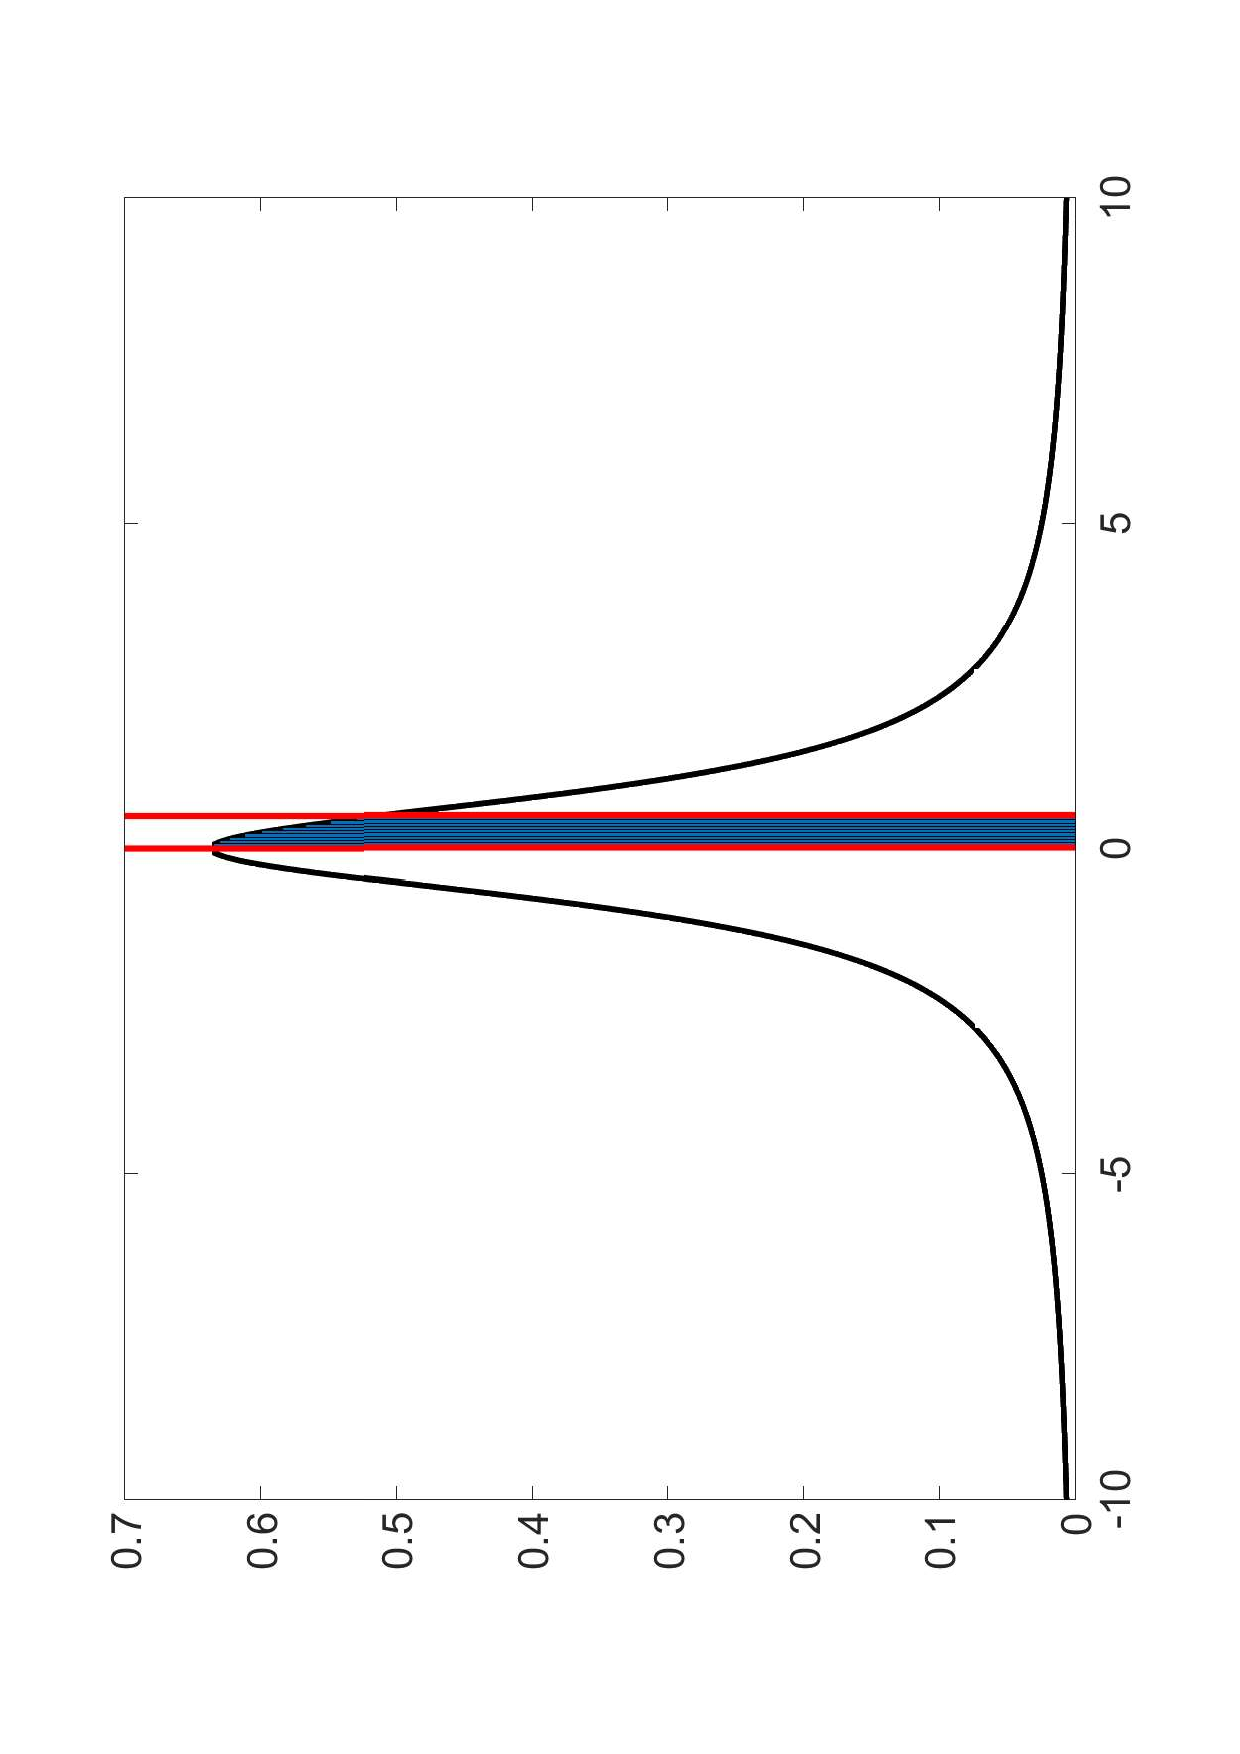
\includegraphics[scale = 0.3, angle = 270]{CauchyPDF4.pdf}
           \caption{Cauchy Distribution Estimator 4}
\end{figure}

\end{frame}

\begin{frame}{Variance}
\begin{columns}[c]
\column{1.0\fullcolwidth}
Question: \\
Under the same sampling size $m$, what is the variance of the estimator above?

\emph{Will they make big difference using different sampling method?}
\column{0\fullcolwidth}
\end{columns}
\end{frame}

\begin{frame}{Variance}
\begin{columns}[c]
\column{1.0\fullcolwidth}
The actual probability $p=0.1476$. According to the variance calculation of the Binomial distribution, the variance of Estimator 1, 2, 3 and 4 are $\frac{0.127}{m}$, $\frac{0.052}{m}$, $\frac{0.0285}{m}$, and $\frac{0.000095}{m}$ respectively ($m$ is the sampling size).\\
From estimator $\hat{p}_{1}$ to estimator $\hat{p}_{4}$, the variance reduction is of order $10^{3}$, which means that the sampling size of $\hat{p}_{1}$ should be $10^{6}$ times more than $\hat{p}_{4}$ to achieve the same precision (Monte Carlo integration error is proportional to $O(N^{-\frac{1}{2}})$.

\emph{What is an effective way to reduce the variance of Monte Carlo Simulation?}
\column{0\fullcolwidth}
\end{columns}
\end{frame}

\begin{frame}{Variance}
\begin{quote}
We have the random variable $\widetilde{f_{n}}(X)$ as a Monte Carlo estimator of $\mathbb{E}(f(X))$. What is the variance of the random variable?\\
If $X$ is discrete,\\
\[ \operatorname{Var}\left(\widetilde{f_{n}}(X)\right)=\frac{\operatorname{Var}(f(X))}{n}=\frac{1}{n} \sum_{x \in \mathcal{X}}[f(x)-\mathbb{E}(f(X))]^{2} p_{X}(x)\]
If $X$ is continuous,\\
\[ \operatorname{Var}\left(\widetilde{f_{n}}(X)\right)=\frac{\operatorname{Var}(f(X))}{n}=\frac{1}{n} \int_{x \in \mathcal{X}}[f(x)-\mathbb{E}(f(X))]^{2} p_{X}(x) d x\]

\end{quote}
\end{frame}

\begin{frame}{Variance}
\begin{quote}

Note that:\\
Typically, we can't calculate the variance directly because $\mathbb{E}\left(\widetilde{f_{n}}(X)\right)$ is unknown and the sum or integral is not feasibly computed. So the definition equations are not very useful for estimating the variance associated with the Monte Carlo estimate.\\ 
We can have an unbiased estimator for $\operatorname{Var}(f(X))$:\\

\[ \widetilde{\operatorname{Var}}\left(\widetilde{f_{n}}(X)\right)=\frac{\widetilde{\operatorname{Var}}(f(X))}{n}=\frac{1}{n(n-1)} \sum_{i=1}^{n}\left(f\left(x_{i}\right)-\widetilde{f_{n}}(x)\right)^{2} \]

\end{quote}

\end{frame}

\begin{frame}{Variance Reduction Methods}

Today we will introduce 3 variance reduction methods:\\
\begin{itemize}
\item Importance Sampling
\item Latin Hypercube Sampling (LHS)
\item Stratified Sampling

\end{itemize}
\end{frame}

\begin{frame}{Importance Sampling}
\begin{definition}
The method we now talk about is called importance sampling because it is based on so-called \textcolor{red}{importance functions}, although it would be more accurate to call it \textcolor{red}{weighted sampling}.\\
In statistics, importance sampling is a general technique for estimating properties of a particular distribution, while only having samples generated from a different distribution than the distribution of interest.
\end{definition}
\end{frame}

\begin{frame}{Importance Sampling}
\begin{definition}
\[E(f(x))=\int f(x)p(x)dx=\int f(x)\frac{p(x)}{q(x)}q(x)dx\]\\ \[E(f(x))\approx \frac{1}{n}\sum_{i=1}^{n}f(x_{i})\frac{p(x_{i})}{q(x_{i})}, x_{i}\sim q\]\\
Let $ w(x_{i}) = \frac{p(x_{i})}{q(x_{i})} $, which is the \textcolor{red}{importance weight} or \textcolor{red}{likelihood ratio}. $q(x_{i})$ is called as \textcolor{red}{proposal distribution} or \textcolor{red}{importance distribution}. $p(x_{i})$ is called as \textcolor{red}{nominal distribution}\\
\[E(f(x))\approx \frac{1}{n}\sum_{i=1}^{n}f(x_{i})w(x_{i})\]
\end{definition}
\end{frame}

\begin{frame}{Importance Sampling}

\begin{block}{What can Importance Sampling be used:}
\begin{itemize}
\item You can sample from original $p$ distribution, but you want to reduce the variance.
\item You can't sample from original $p$ distribution, and you have to choose a $q$ distribution that is close enough to $p$ distribution.
\end{itemize}
\end{block}

\end{frame}

\begin{frame}{Importance Sampling Variance}

Let $\mu=\int_{\mathcal{D}} f(\boldsymbol{x}) p(\boldsymbol{x}) \mathrm{d} \boldsymbol{x}$ and $q(x)>0$ whenever $f(\boldsymbol{x}) p(\boldsymbol{x}) \neq 0$. Then $\mathbb{E}_{q}\left(\hat{\mu}_{q}\right)=\mu$, and $\operatorname{Var}_{q}\left(\hat{\mu}_{q}\right)=\sigma_{q}^{2} / n$ where\\
\[\sigma_{q}^{2}=\int_{\mathcal{D}} \frac{(f(\boldsymbol{x}) p(\boldsymbol{x}))^{2}}{q(\boldsymbol{x})} \mathrm{d} \boldsymbol{x}-\boldsymbol{\mu}^{2}\]
\[=\int_{\mathcal{D}} \frac{(f(\boldsymbol{x}) p(\boldsymbol{x})-\mu q(\boldsymbol{x}))^{2}}{q(\boldsymbol{x})} \mathrm{d} \boldsymbol{x}\]

\end{frame}

\begin{frame}{Proof}

Using $Q=\{\boldsymbol{x} | q(\boldsymbol{x})>0\}$. We find that,\\
\[\operatorname{Var}_{q}\left(\hat{\mu}_{q}\right)=\frac{1}{n}\left[\int_{Q}\left(\frac{f(\boldsymbol{x}) p(\boldsymbol{x})}{q(\boldsymbol{x})}\right)^{2} q(\boldsymbol{x}) \mathrm{d} \boldsymbol{x}-\mu^{2}\right]\]
\[=\int_{\mathcal{D}} \frac{(f(\boldsymbol{x}) p(\boldsymbol{x})-\mu q(\boldsymbol{x}))^{2}}{q(\boldsymbol{x})} \mathrm{d} \boldsymbol{x}\]
Because the contribution to the integral from $x$ in $\mathcal{D} \cap \mathcal{Q}^{c}$ and $\mathcal{Q} \cap \mathcal{D}^{c}$ are zero. Simple arrangements give the two forms in $\sigma_{q}^{2}$\\


\end{frame}

\begin{frame}{Confidence Interval}

First, estimate $\sigma_{q}^{2}$. From the second expression of $\sigma_{q}^{2}$, we find that,\\
\[\sigma_{q}^{2}=\mathbb{E}_{q}\left((f(\boldsymbol{X}) p(\boldsymbol{X})-\mu q(\boldsymbol{X}))^{2} / q(\boldsymbol{X})^{2}\right)\]
Because $x_{i}$ are sampled from $q$, the natural variance estimate is:\\
\[\hat{\sigma}_{q}^{2}=\frac{1}{n} \sum_{i=1}^{n}\left(\frac{f\left(\boldsymbol{x}_{i}\right) p\left(\boldsymbol{x}_{i}\right)}{q\left(\boldsymbol{x}_{i}\right)}-\hat{\boldsymbol{\mu}}_{q}\right)^{2}=\frac{1}{n} \sum_{i=1}^{n}\left(w_{i} f\left(\boldsymbol{x}_{i}\right)-\hat{\boldsymbol{\mu}}_{q}\right)^{2}\]
where $w_{i}=p\left(\boldsymbol{x}_{i}\right) / q\left(\boldsymbol{x}_{i}\right)$. Then an approximation $99 \%$ confidence inter for $\mu$ is $\hat{\mu}_{q} \pm 2.58 \hat{\sigma}_{q} / \sqrt{n}$.

\end{frame}

\begin{frame}{Choice of $q$}

The first expression:\\
\[\sigma_{q}^{2}=\int_{\mathcal{D}} \frac{(f(\boldsymbol{x}) p(\boldsymbol{x}))^{2}}{q(\boldsymbol{x})} \mathrm{d} \boldsymbol{x}-\boldsymbol{\mu}^{2}\]
A better $q$ is one that gives a smaller value of $\int_{\mathcal{D}}(f p)^{2} / q \mathrm{d} \boldsymbol{x}$. When we want upper bounds on $\sigma_{q}^{2}$, we can bound $\int_{\mathcal{D}}(f p)^{2} / q \mathrm{d} \boldsymbol{x}$.

\end{frame}

\begin{frame}{Choice of $q$}

The second expression:\\
\[\sigma_{q}^{2}=\int_{\mathcal{D}} \frac{(f(\boldsymbol{x}) p(\boldsymbol{x})-\mu q(\boldsymbol{x}))^{2}}{q(\boldsymbol{x})} \mathrm{d} \boldsymbol{x}\]
The numerator in the integral at the right is small when $f(\boldsymbol{x}) p(\boldsymbol{x})-\mu q(\boldsymbol{x})$ is close to zero, that is, when $q(x)$ is nearly proportional to $f(x)p(x)$. From the denominator, we see that regions with small values of $q(x)$ greatly magnify whatever lack of proportionality appears in the numerator.

\end{frame}


\begin{frame}{Choice of $q$}
\begin{quote}

Proportionality is wonderful, but it never happens! Because once it happens, it implies that the original integral involving $p(x)$ is computable and hence there is no reason to do Monte Carlo at all...

\end{quote}
\end{frame}

\begin{frame}{Choice of $q$}

In general, the density $q^{*}$that minimizes $\sigma_{q}^{2}$ is proportional to $|f(x)| p(x)$, outside of trivial cases where $\int|f(x)| p(x) \mathrm{d} x=0$.\\
Let's prove that $q^{*}(x)=|f(x)| p(x) / \mathbb{E}_{p}(|f(X)|)$ is optimal.

\end{frame}

\begin{frame}{Choice of $q$}

\textcolor{red}{Cauchy-Schwarz Inequality}
Let $q$ be any density that is positive when $f p \neq 0$. Then,\\
\[\mu^{2}+\sigma_{q^{*}}^{2}=\int \frac{f(\boldsymbol{x})^{2} p(\boldsymbol{x})^{2}}{q^{*}(\boldsymbol{x})} \mathrm{d} \boldsymbol{x}=\int \frac{f(\boldsymbol{x})^{2} p(\boldsymbol{x})^{2}}{|f(\boldsymbol{x})| p(\boldsymbol{x}) / \mathbb{E}_{p}(|f(\boldsymbol{X})|)} \mathrm{d} \boldsymbol{x}\]
\[=\mathbb{E}_{p}(|f(\boldsymbol{X})|)^{2}=\mathbb{E}_{q}(|f(\boldsymbol{X})| p(\boldsymbol{X}) / q(\boldsymbol{X}))^{2}\]
\[\leqslant \mathbb{E}_{q}\left(f(\boldsymbol{X})^{2} p(\boldsymbol{X})^{2} / q(\boldsymbol{X})^{2}\right)=\mu^{2}+\sigma_{q}^{2}\]
So, $\sigma_{q^{*}}^{2} \leqslant \sigma_{q}^{2}$.

\end{frame}

\begin{frame}{Importance Sampling}

\begin{block}{$q(x)$ Wish-list:}
\begin{itemize}
\item $q(x)>0$ for any $f(x)p(x) \neq 0$.
\item $q(x)$ should be close to being proportional to $|f(x)p(x)|$.
\item It should be easy to sample from $q(x)$.
\item $q(x)$ should be easy to compute for any value $x$ that might realize.
\end{itemize}
\end{block}

\end{frame}

\begin{frame}{Choice of $q$}



\begin{figure}[ht]
		  \centering
          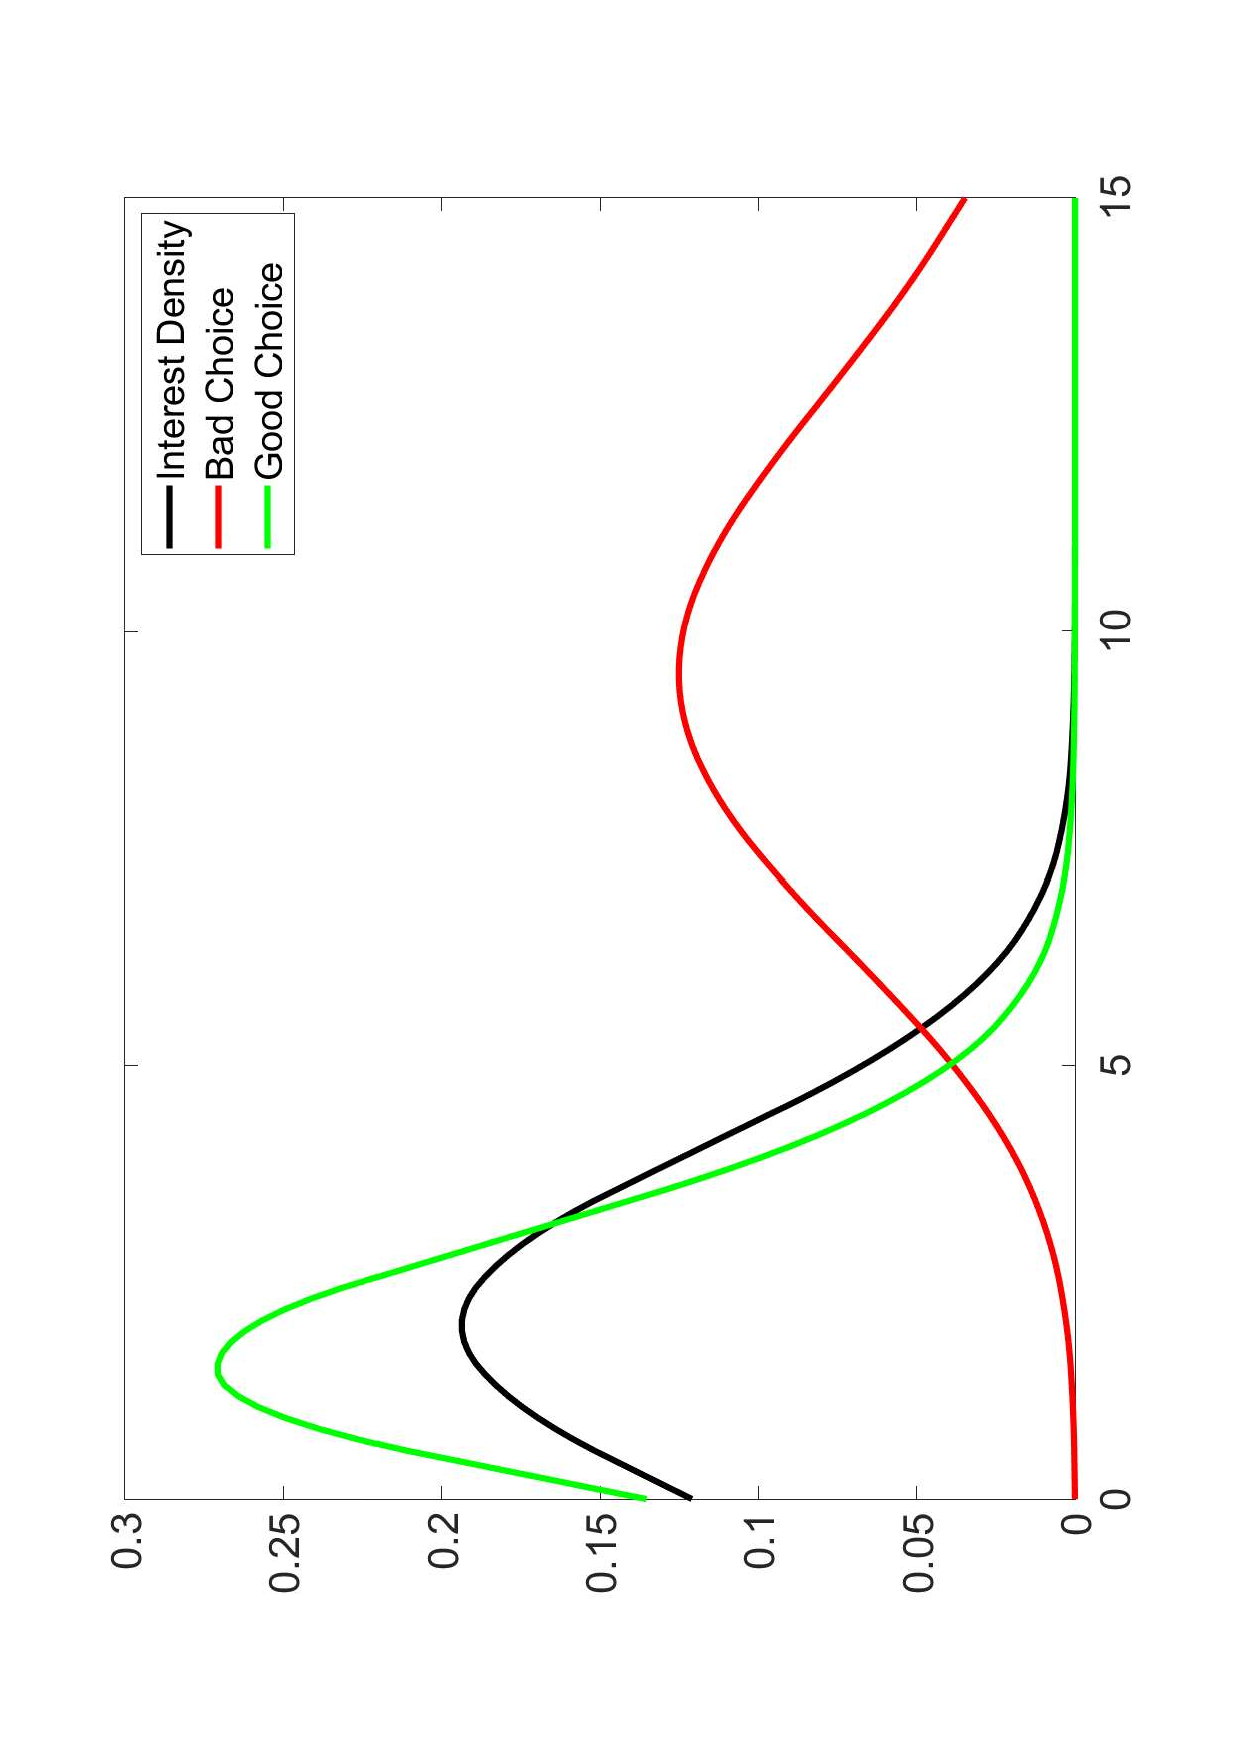
\includegraphics[scale = 0.3, angle=270]{Comparison.pdf}
           \caption{Good and Bad Choice of $q$ Density}
 \end{figure}

On the contrary, the bad choice of $q$ density will increase the variance.
\end{frame}

\begin{frame}{Example of Choosing $q$}

Now, let's use the likelihood ratio $w(\boldsymbol{x})=p(\boldsymbol{x}) / q(\boldsymbol{x})$ as a means to understand which importance sampling densities are good or bad choices. The first term in $\sigma_{q}^{2}$ is $\int f(x)^{2} p(x)^{2} / q(x) \mathrm{d} x$. Write the term as\\
\[\mathbb{E}_{p}\left(f(\boldsymbol{X})^{2} w(\boldsymbol{X})\right)=\mathbb{E}_{q}\left(f(\boldsymbol{X})^{2} w(\boldsymbol{X})^{2}\right)\]The appearance of $q$ in the denominator of $w$, means that light tailed importance densities $q$ are dangerous. One smart idea is that $f$ should be small just where it needs to be to offset the small denominator. However, we often need to use the same sample with multiple integral. \\
\textcolor{red}{So, as a rule, $q$ should have tails at least as heavy as $p$ does.}


\end{frame}

\begin{frame}{Example of Choosing $q$}

When $p$ is a Gaussian distribution, then a common tactic is to take $q$ to be a student's $t$ distribution. Such a $q$ has heavier tails than $p$. It even has heavier tails than $fp$ for integral of the form $f(\boldsymbol{x})=\exp \left(\boldsymbol{x}^{\top} \theta\right)$ (Proportional to another Gaussian density).\\
But, the reverse practice of using Gaussian importance distribution $q$ for a student's $t$ nominal distribution, can easily lead to $\sigma_{q}^{2}=\infty$. The infinite variance could be largely attributable to the unimportant region of $\mathcal{D}$ where $|f| p$ is small, where $q$ is extremely small.

\end{frame}

\begin{frame}{Importance Sampling}
\begin{block}{Importance Sampling Algorithm:}
\begin{itemize}
\item Draw $N$ samples from $q$.
\item Calculate the probability of each sample.
\item Evaluate $p$ over the N samples.
\item Calculate the importance weights $w=p / q$.
\item Draw $N$ samples from $g$ with new weight $w$.
\end{itemize}
\end{block}

\end{frame}

%%% Local Variables:
%%% mode: latex
%%% TeX-master: "probability-main"
%%% End:


 \section{Example of Importance Sampling}
\outlinechapter{Independence Study: Importance Sampling}
 \subsection{Example of Importance Sampling}

\begin{frame}{Example of Importance Sampling -- Estimate Distribution}

Estimate the Beta Function -- $beta(2, 11)$, and suppose we do not know the equation. \\
We have two proposal options:\\
(1) Uniform Distribution;\\
(2) $beta(2,11)$ distribution itself.

\end{frame}

\begin{frame}{Example of Importance Sampling -- Estimate Distribution}
\begin{figure}[ht]
		  \centering
          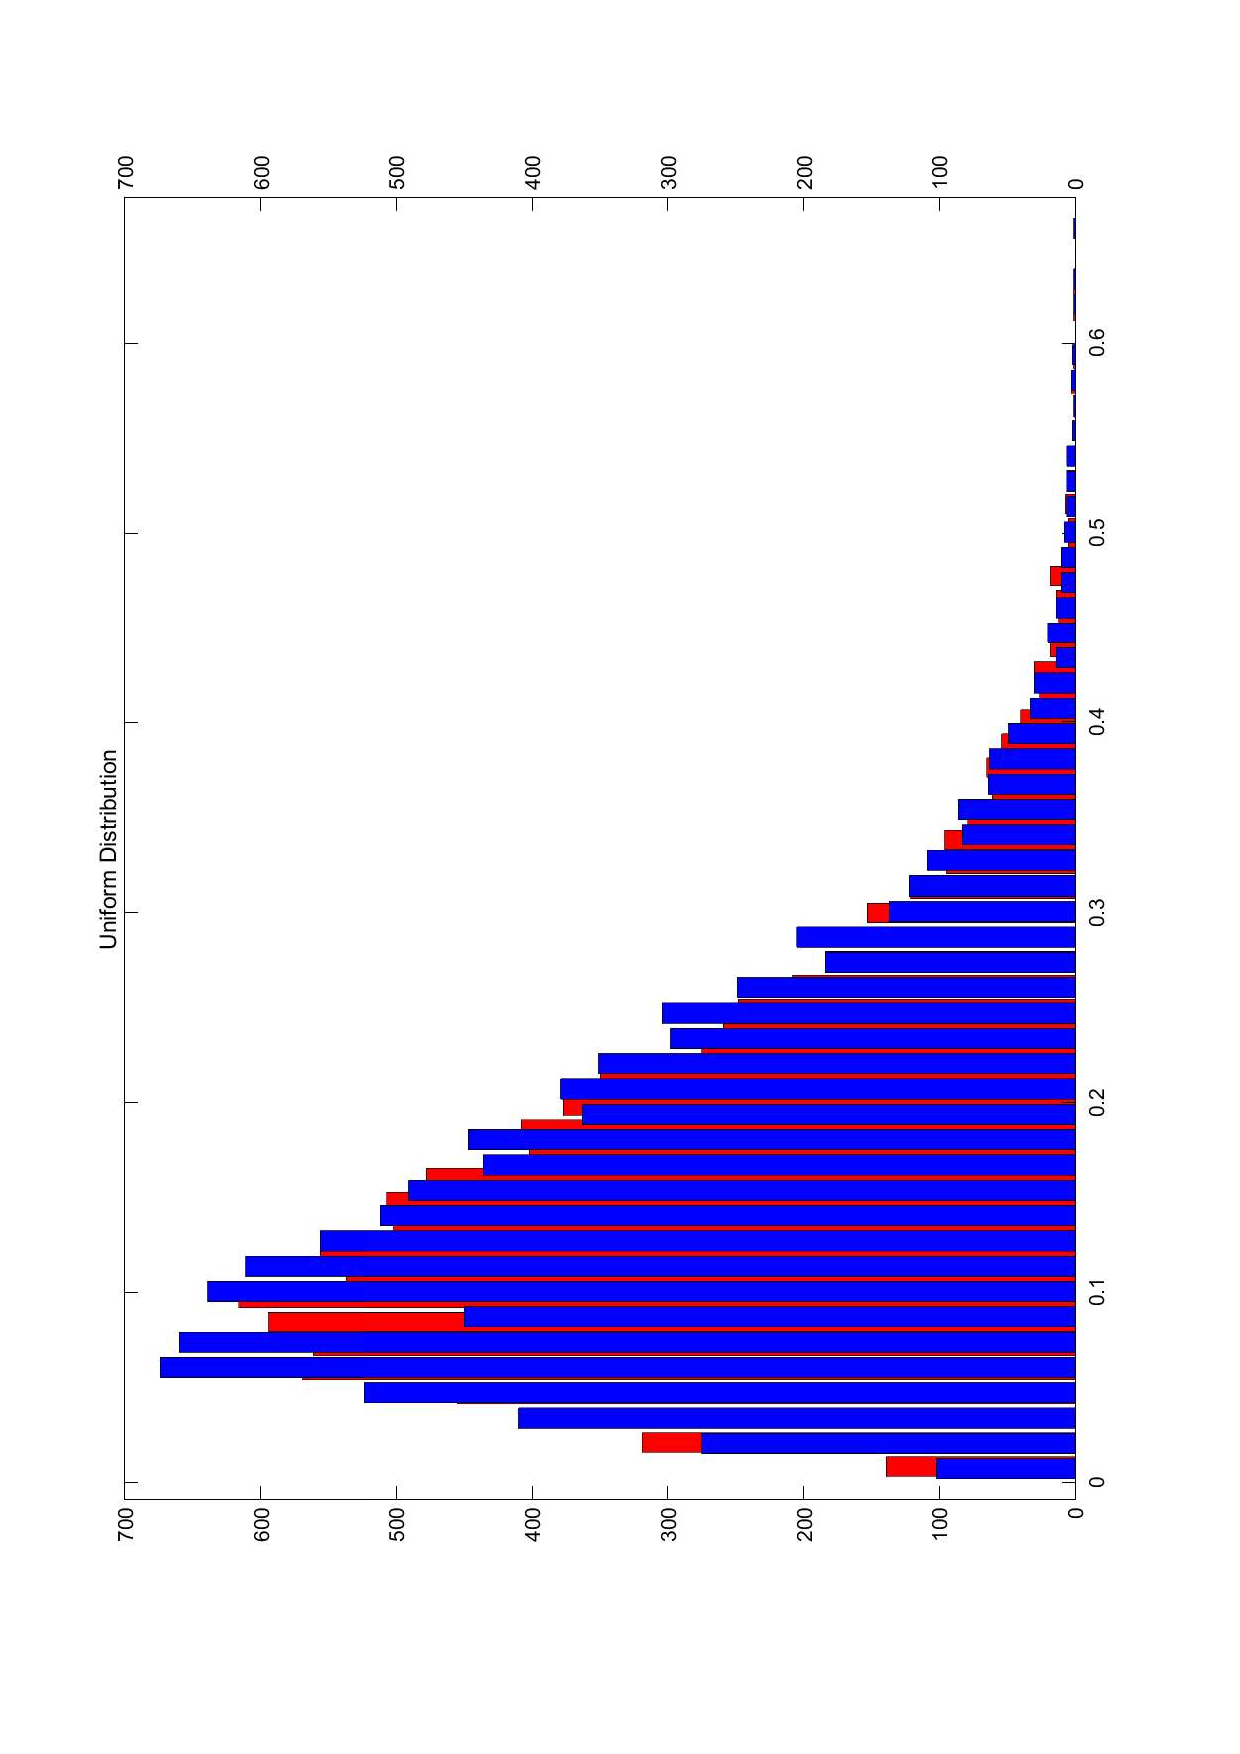
\includegraphics[scale = 0.3, angle=270]{UniformSimulation.pdf}
           \caption{Estimation using Uniform Distribution}
 \end{figure}
\end{frame}

\begin{frame}{Example of Importance Sampling -- Estimate Distribution}
\begin{figure}[ht]
		  \centering
          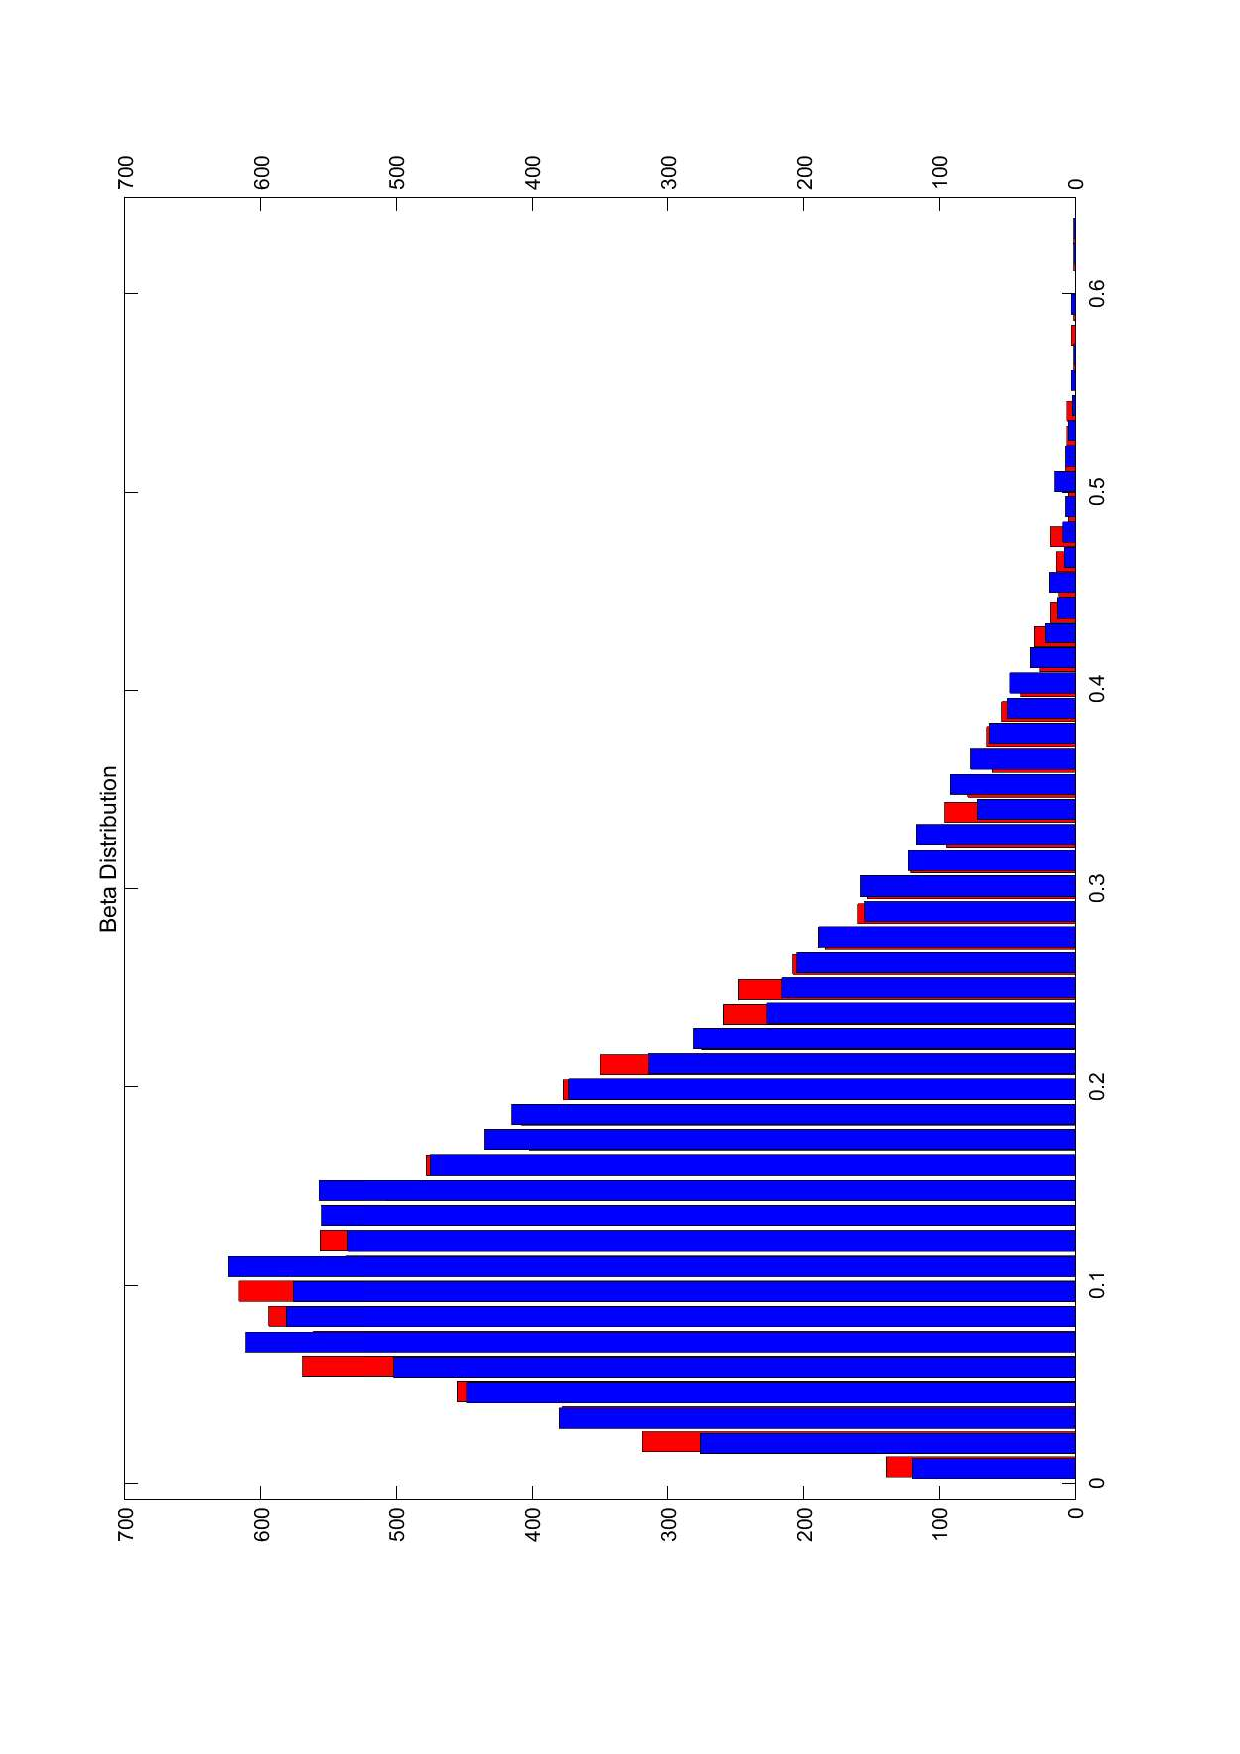
\includegraphics[scale = 0.3, angle=270]{BetaSimulation.pdf}
           \caption{Estimation using Beta Distribution}
 \end{figure}
\end{frame}

\begin{frame}{Example of Importance Sampling -- Calculate Probability}
\begin{example}
Get the expectation value for the function $f(x)$ below, with $x$ value drawn from a standard normal $p(x)=N(0,1)$. \\
\[f(x)=10 e^{-5(x-3)^{4}}\]
\[p(x)=\frac{1}{\sqrt{2 \pi}} e^{-x^{2} / 2}\]First, we calculate the theoretical expectation value using Wolfram Alpha:\\
\[\int_{-\infty}^{\infty} 5 e^{(-3+x)^{4}-\frac{x^{2}}{2}} \sqrt{\frac{2}{\pi}} d x \approx 0.089392379460790\]
\end{example}
\end{frame}

\begin{frame}{Direct Monte Carlo}
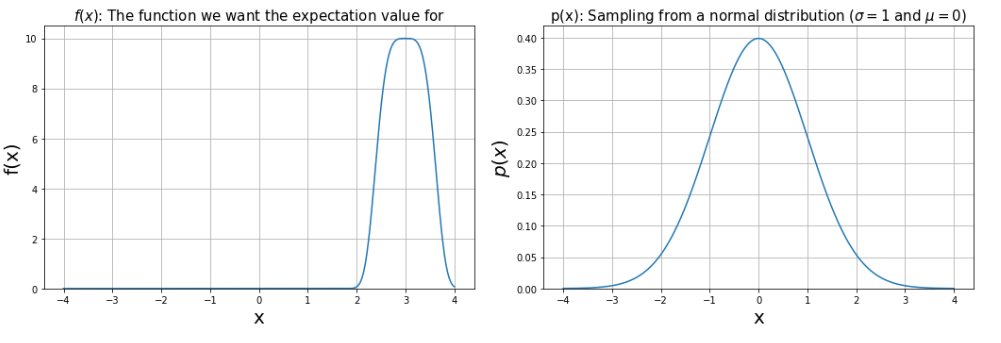
\includegraphics[width=\textwidth*\real{\figfactor}]{ExampleP.png}\\
From the figure above, it's obvious that \textcolor{red}{very few} of the values sampled from $p(x)$ will fall inside the high-value range of the $f(x)$.\\
For $500$ times Monte Carlo simulation:\\
The average expectation value is $0.08920550043488344$.\\
The standard deviation in the average expectation value is $0.024553920882104115$.
\end{frame}

\begin{frame}
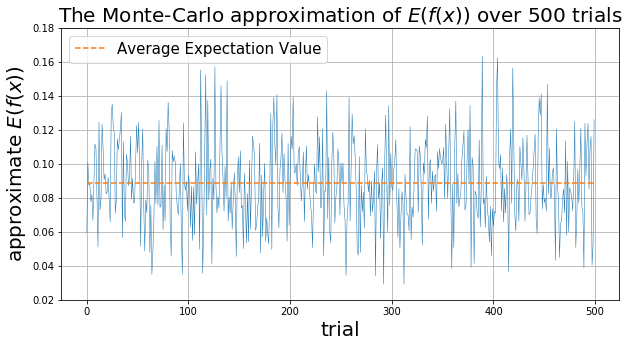
\includegraphics[width=\textwidth*\real{\figfactor}]{DirectMCVariance.png}\\
\end{frame}

\begin{frame}{Importance Sampling}
Now, we choose the second probability density function, $q(x)$, from which sample values are more likely to fall within the high-value range of $f(x)$.\\
For $500$ times Monte Carlo simulation:\\
The average expectation value is $0.0894449539169$.\\
The standard deviation in the average expectation value is $0.00370078677103$.

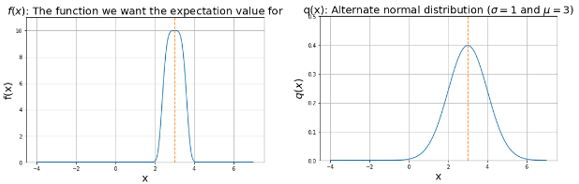
\includegraphics[width=\textwidth*\real{\figfactor}]{q.png}\\
\end{columns}
\end{frame}

\begin{frame}
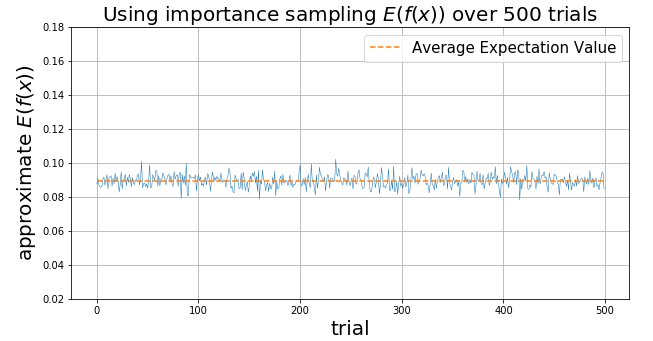
\includegraphics[width=\textwidth*\real{\figfactor}]{ImporSamVariance.png}\\
\end{frame}

\begin{frame}{Pitfall}
\begin{quote}
\textcolor{red}{The tails of the distributions matters!}\\
\end{quote}
While $q(x)$ might be roughly the similar shape as $p(x)$, serious difficulties arise if $q(x)$ gets small much faster than $p(x)$ out in the tail. In such a case, although it is less possible that you will sample a value of $x_{i}$ from the far tails of $q(x)$, your Monte Carlo estimator will take $g\left(x_{i}\right) / h\left(x_{i}\right)$ for such $x_{i}$ may be orders of magnitude larger than the regular values $g\left(x\right) / h\left(x\right)$.
\end{frame}

\begin{frame}{Comparison}
\begin{quote}
\textcolor{red}{Importance Sampling} and \textcolor{red}{Acceptance/Rejection Algorithm} are quite similar ideas. Both of them distort a sample from one distribution in order to sample from another. \\
What is the difference of \textcolor{red}{Importance Sampling} and \textcolor{red}{Acceptance/Rejection Algorithm}?\\
\end{quote}
\end{frame}

\begin{frame}{More Advanced Importance Sampling}
\begin{itemize}
\item Adaptive parametric Importance Sampling.
\item Sequential Importance Sampling.
\item Annealed Importance Sampling
\item SIS with Re-sampling.
\item SIS and Markov Chain Sampling
\end{itemize}
\end{frame}

\begin{frame}{Stratified Sampling    \href{https://en.wikipedia.org/wiki/Stratified_sampling}{[2]}}

 In statistical surveys, when sub-populations within an overall population vary, it could be advantageous to sample each sub-population (stratum) independently. Stratification is the process of dividing members of the population into homogeneous subgroups before sampling. \\
 \textcolor{red}{Mutually Exclusive}: every element in the population must be assigned to only one stratum.\\
 \textcolor{red}{Collectively Exclusive}: no population element can be excluded.
 
\end{frame}

\begin{frame}{Stratified Sampling Procedure}

 1. Divide the population into strata, or groups of individuals that are similar (or homogeneous) in some way that is important to the response.\\
 2. Choose a separate simple random sample (SRS) from each stratum.\\
 3. Combine these SRS's to form a stratified random sample.
 
\end{frame}

\begin{frame}{Stratified Sampling -- Advantages and Disadvantages}

\textcolor{red}{Advantages}:
\begin{itemize}

\item If measurements within strata have lower standard deviation, stratification gives smaller error in estimation.
\item For many applications, measurements become more manageable and/or cheaper when the population is grouped into strata.
\item It is often desirable to have estimates of population parameters for groups within the population
\end{itemize}
\textcolor{red}{Disadvantages}:
Stratified sampling is not useful when the population cannot be exhaustively partitioned into disjoint subgroups.
\end{frame}

\begin{frame}{Stratified Sampling -- Mean and s.d.}

Mean:\\
\[\overline{x}=\frac{1}{N} \sum_{h=1}^{L} N_{h} \overline{x_{h}}\]
Standard error:\\
\[s_{\overline{x}}^{2}=\sum_{h=1}^{L}\left(\frac{N_{h}}{N}\right)^{2}\left(\frac{N_{h}-n_{h}}{N_{h}}\right) \frac{s_{h}^{2}}{n_{h}}\]
Where, $L$ -- Number of strata; $N$ -- the sum of all stratum sizes; $N_{h}$ -- Size of stratum $h$; $\overline{x}_{h}$ -- Sample mean of stratum $h$; $n_{h}$ -- Number of observations in stratum $h$; $s_{h}$ -- Sample standard deviation of stratum $h$.

\end{frame}

\begin{frame}{Stratified Sampling -- Example}

For proportional allocation strategy, the size of the sample in each stratum is taken in proportion to the size of the stratum. Suppose that in a company there are the following staff:
\begin{itemize}

\item male, full-time: $90$
\item male, part-time: $18$
\item female, full-time: $9$
\item female, part-time: $63$
\end{itemize}
Now we want to take sample of 40 staff, stratified according to the above categories.

\end{frame}

\begin{frame}{Stratified Sampling -- Example}
\begin{itemize}

\item male, full-time $=90 \times(40 \div 180)=20$
\item male, part-time $=18 \times(40 \div 180)=4$.
\item female, full-time $=9 \times(40 \div 180)=2$.
\item female, part-time $=63 \times(40 \div 180)=14$.
\end{itemize}

\end{frame}

\begin{frame}{Stratified Sampling -- Example}

\begin{figure}[ht]
		  \centering
          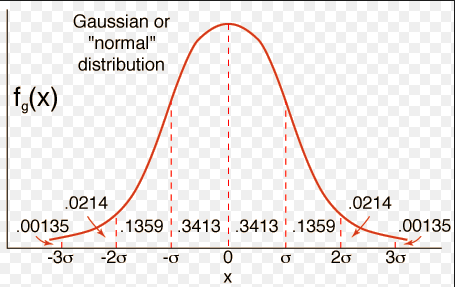
\includegraphics[scale = 0.4]{Normal.png}
           \caption{Gaussian Distribution}
           \href{http://hyperphysics.phy-astr.gsu.edu/hbase/Math/gaufcn.html}{Image Source: Rohlf}
 \end{figure}
 
 If we want to sample $10000$ from the Gaussian distribution above, the sample size in different interval should be:\\
 $[-\infty, -3\sigma]$: $14$; $[-3\sigma, -2\sigma]$: $214$; $[-2\sigma,-\sigma]$: $1359$; $[-\sigma,0]$: $3413$;\\
 $[0,\sigma]$:$3413$; $[\sigma,2\sigma]$:$1359$; $[2\sigma,3\sigma]$: $214$; $[3\sigma, +\infty]$: $14$.
 
 \end{frame}

\begin{frame}{Latin Hypercube Sampling}
Purpose:\\
Recreate the input distribution through less samples.\\
Method:\\
\begin{itemize}
\item The key to this method is \textcolor{red}{stratification} of the input probability distribution.
\item Stratification \textcolor{red}{divides the cumulative curve} into \textcolor{red}{equal} intervals.
\item A sample is then \textcolor{red}{randomly} taken from each interval or "stratification".
\end{itemize}
\end{frame}

\begin{frame}{LHS -- One Dimension}
\begin{figure}[ht]
		  \centering
          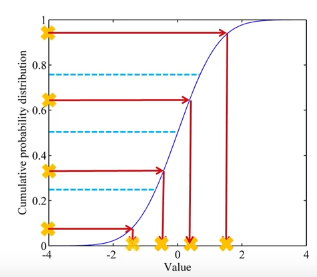
\includegraphics[scale = 0.6]{LHS1D.png}
           \caption{One-dimensional LHS}
           \href{https://www.youtube.com/watch?v=H0RZ1uezuuw}{Image Source: Iman}
 \end{figure}
 Only one sample per stratification.
\end{frame}

\begin{frame}{LHS -- Two Dimension}

 In the context of statistical sampling, a square grid containing sample position is a \textcolor{red}{Latin Square} if and only if there is only \textcolor{red}{one sample} in each row and each column.\\
 A \textcolor{red}{Latin Hypercube} is the generalization of this concept to an arbitrary number of dimensions, whereby each sample is the only one in each axis-aligned heperplane containing it.
 
\end{frame}

\begin{frame}{Comparison}

 \textcolor{red}{Monte Carlo Method -- Memory-less:}\\
 New sample points are generated without taking into account the previously generated sample point. \\
 \textcolor{red}{Latin Hypercube Sampling -- Memory:}\\
 The row and the column the sample point was taken has to be considered to generate the new data points. Spread sample points 'more uniformly' across all the possible values than the basic Monte Carlo methods.
 
\end{frame}

\begin{frame}{LHS -- One Dimension}
\begin{figure}[ht]
		  \centering
          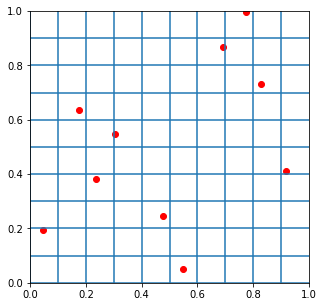
\includegraphics[scale = 0.4]{LHS2D.png}
           \caption{Two-dimensional LHS}
 \end{figure}
 Only one sample in each row and each column.
\end{frame}

\begin{frame}{Reference}
\begin{thebibliography}
\bibitem{[1]} Robert, C., & Casella, G. Monte Carlo statistical methods. Springer Science & Business Media, 2013:  90-91.
\end{thebibiliography}
\end{frame}
%%% Local Variables:
%% y-main"
%%% End:




\end{document}


% Templates
\begin{frame}{}
\begin{itemize}
\item
\end{itemize}
\end{frame}

\begin{frame}{}
\begin{columns}
\column{0.5\fullcolwidth}

\column{0.5\fullcolwidth}
% \includegraphics[width=1\textwidth*\real{\figfactor}]{fig-lorenz-63.png}
\end{columns}
\end{frame}



%%% Local Variables:
%%% mode: latex
%%% TeX-master: t
%%% End:
